\documentclass[twoside,11pt]{article}
\usepackage{amssymb,amsmath, amsfonts,latexsym,mathtext, array, graphicx, geometry, caption, subcaption}
\geometry{margin=1.5cm}
\setlength{\parskip}{0.8ex plus 0.1ex minus 0.2ex}
\newcommand{\M}[1]{\boldsymbol{\mathbf{#1}}}
\newcommand{\V}{\M}
\newcommand{\Cal}{\mathcal}

\newtheorem{thm1}{Theorem}
\newtheorem{def1}{Definition}

\begin{document}

\title{Machine Learning 6.867 - Pset 1}

\maketitle
%!TEX root = pset1.tex

\section{Implement Gradient Descent}\label{sec:grad_desc}

\subsection{Gradient Descent Implementation}
We implemented a basic gradient descent function in MATLAB. In this function, the user can specify the objective function and the corresponding gradient function. User also specify initial guess, the constant step size, and the convergence threshold. \\
The procedure works as the following: starting at the initial guess, we move to a new point by taking a step (of the specified step size) in the direction of the gradient. We repeat the process until the objective values between two iterations are less than the specified threshold.

\subsection{Testing Gradient Descent}
We test the gradient descent procedure in the following functions:
\begin{enumerate}
\item $f(x_1, x_2) = 3x_1^2 + 2x_1x_2 + x_2^2 - 4x_1 + 5x_2$ (By completing the square we get the optimal value is at $x_1 = 2.25, x_2 = -4.75$.)
\item $f(x) = -\frac{1}{\sqrt{2\pi}\sigma}e^{-(x-\mu)^2/2\sigma^2}$ (negative of a Gaussian pdf, with $\mu = 0$ and $\sigma = 1$.)
\item $f(x) = x^3 - 10x$. (This is not a convex function; local minimum is at $1.8257$ and global minimum is negative infinity).
\end{enumerate}

The basic gradient descent method works decently well in the first two functions. In most specifications of the initial guess and step size the procedure converges to the right answer. Changing the convergence threshold to very large gives imprecise results, and changing it to very small results in more iterations until convergence. In some cases, very large or very small step sizes may result in non-convergence. In the third function which is non-convex, the initial guess can lead us to the incorrect, local minimum.  

\begin{figure}[h!]
\centering
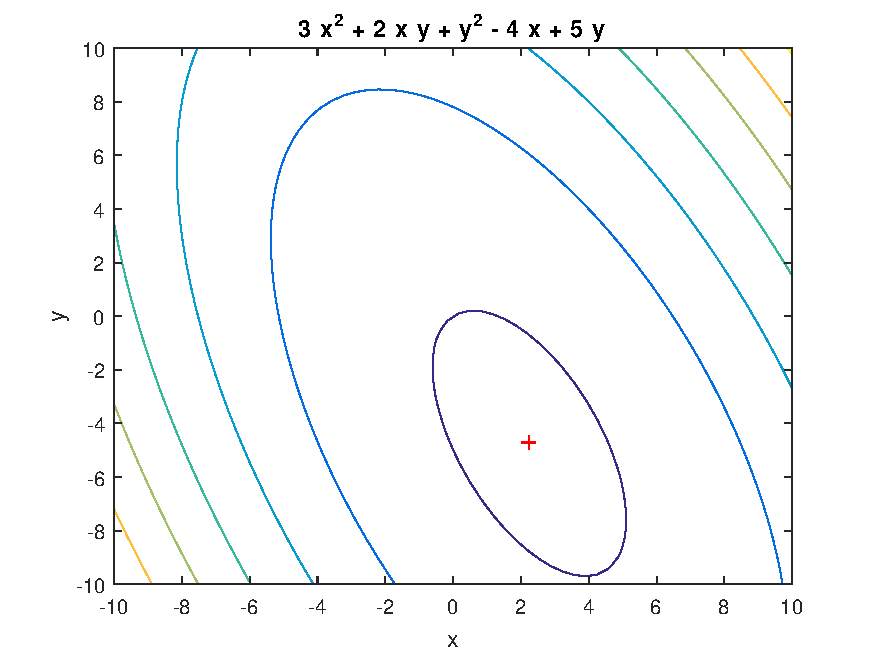
\includegraphics[scale=0.4]{hw1_1.pdf}
\caption{Contour plot of the first function. The gradient descent method moves to the red cross where the local/global optimal is.}
\end{figure}


\subsection{Numerical Gradient}
We can also numerically evaluate the gradient at a given point. The partial derivative at $x_i$ is evaluated by taking the difference between $f(\V x+\V h)$ and $f(\V x-\V h)$, where $\V h$ is the vector of all zeros except for the $i$th component being $\epsilon$, and divide the difference by $2\epsilon$. We apply this numerical gradient in place of the analytic one in the original three functions, and found that for sufficiently small $\epsilon$, the results are almost identical!

\subsection{Comparing with Sophisticated Methods}
As the final step to evaluate our implementation of gradient descent, we would like to compare ours with the more developed methods. Comparing with \texttt{fminunc}, our implementation is dramatically slower, unfortunately. For example, for the same convergence criterion, it takes 8 iterations for \texttt{fminunc} to converge, whereas it takes 35 iterations for our method. We think the disadvantage is from our constant step size. Since this size does not adapt to where we are, our method is likely to undershoot or overshoot. An improvement could be using backtracking, exact line-search, etc. methods to adaptively update the step size.  
%!TEX root = pset1.tex

\section{Linear Basis Function Regression}\label{sec:lin_basis_fn_reg}
%!TEX root = pset1.tex

\section{Ridge Regression}\label{sec:ridge_reg}

\subsection{Implementation}
Ridge regression is the particular case of regularized least squares with a quadratic regularizer term.  The error function that we aim to minimize over is given by:
\begin{equation} \label{eq:ridge_error_fn}
\frac{1}{2} \sum_{n=1}^{N} (t_n - \M{w}^T \phi (\M{x}_n) )^2 + \frac{\lambda}{2} \M{w}^T \M{w}
\end{equation}

The closed-form solution of this problem is well-known, and can be derived by setting the gradient of (\ref{eq:ridge_error_fn}) equal to zero.  The optimal solution for $\M{w}$ is provided by Bishop (2006), page 145:

\begin{equation} \label{eq:ridge_sol}
\M{w} = (\lambda \M{I} + \Phi^T \Phi)^{-1} \Phi^T \M{t}
\end{equation}

% Reference: Bishop (2006), pages 144-145


%!TEX root = pset1.tex

\section{Sparsity and LASSO}\label{sec:gen}
An alternative approach is to use the $L_1$ norm regularizer in the objective for regularized least squares.  The error function that we aim to minimize over is given by:
\begin{equation} \label{eq:lasso_error_fn}
\frac{1}{2} \sum_{n=1}^{N} (t_n - \M{w}^T \phi (\M{x}_n) )^2 + \frac{\lambda}{2} \sum_{j=1}^{M} |w_j|
\end{equation}

The LASSO is widely used in practice because it leads to solutions which are relatively sparse, i.e. the resulting prediction vector $\M{w}$ tends to have few non-zero components.  

To test this method and its sparsity properties, we consider a regression problem with 5 training points and 500 testing points in $\mathbb{R}^{12}$.  The data is generated according to  $f(x) = \M{w}^T \phi (\M{x}) + \epsilon$, where $\epsilon \sim  N(0,\sigma^2)$ and $\M{w} \in \mathbb{R}^{12}$ is a sparse vector with only two non-zero components.  For this problem, we assume that $\M{w}$ is unknown, and we estimate this vector with ridge regression in Section~\ref{sec:sparsity_ridge_reg} and with LASSO in Section~\ref{sec:sparsity_grad_desc}.  Let $\lambda_2$ denote the regularizer term for the $L_2$ norm and let $\lambda_1$ denote the regularizer term for the $L_1$ norm.  Figure~\ref{fig:lasso_sparsity} shows plots of the estimated function with different regularizers.  

\subsection{Ridge Regression Gradient Descent} \label{sec:sparsity_ridge_reg}
Applying our method for gradient descent to the ridge regression problem on the training dataset of 12 points, we compute the vector of weights $\M{w}$ and MSE on the testing dataset for $\lambda_2 = 0.1$.  We obtain: 
%
\begin{flalign*}
\M{w} &= (0.12,0.14,0.22,0.20,0.09,-0.05,-0.20,-0.30,-0.32,-0.25,-0.08,0.12)\\
\text{MSE} &=  0.2606.
\end{flalign*}
%
If we disable the $L_2$ regularizer (set $\lambda_2 = 0$), i.e., the OLS estimator, we obtain:
%
\begin{flalign*}
\M{w} &= (1.15,1.30,1.72,0.67,-1.73,-4.28,-5.16,-3.27,0.48,3.01,0.61,-8.83),\\
\text{MSE} &=  109.2910.
\end{flalign*}
%
\subsection{LASSO Gradient Descent} \label{sec:sparsity_grad_desc}
Similarly, we apply our method for gradient descent to the LASSO problem on the on the training dataset of 12 points.  For $\lambda_1 = 0.1$, we find: 
%
\begin{flalign*}
\M{w} &= (0.00,0.00,0.43,0.00,0.00,-0.00,-0.00,-0.00,-1.02,-0.00,-0.00,0.00),\\
\text{MSE} &=0.0487.
\end{flalign*}

\subsection{Sparsity Properties of LASSO}
We observe from Figure \ref{fig:lasso_sparsity} and MSE values that the LASSO estimation is closest to the true generating function, compared to ridge regression or non-regularized OLS. In terms of sparsity, the LASSO estimator has only two variables that are non-zero (the rest are within numerically negligible deviation from 0), whereas the other estimators lead to non-sparse results. The $L_0$ norm regularizer, which penalizes based on the number of non-zero elements in $\V w$, is the true sparsity regularizer; however, this leads to a problem which is non-convex and difficult to solve directly.  Because the $L_1$ norm is the convex hull of the $L_0$ norm, LASSO can be used as an approximation to often give sparse results. Even though the $L_2$ norm regularization penalizes the size of $\V w$, due to the geometry of the norm it does not provide sparse results.


\begin{figure}[h!]
\centering
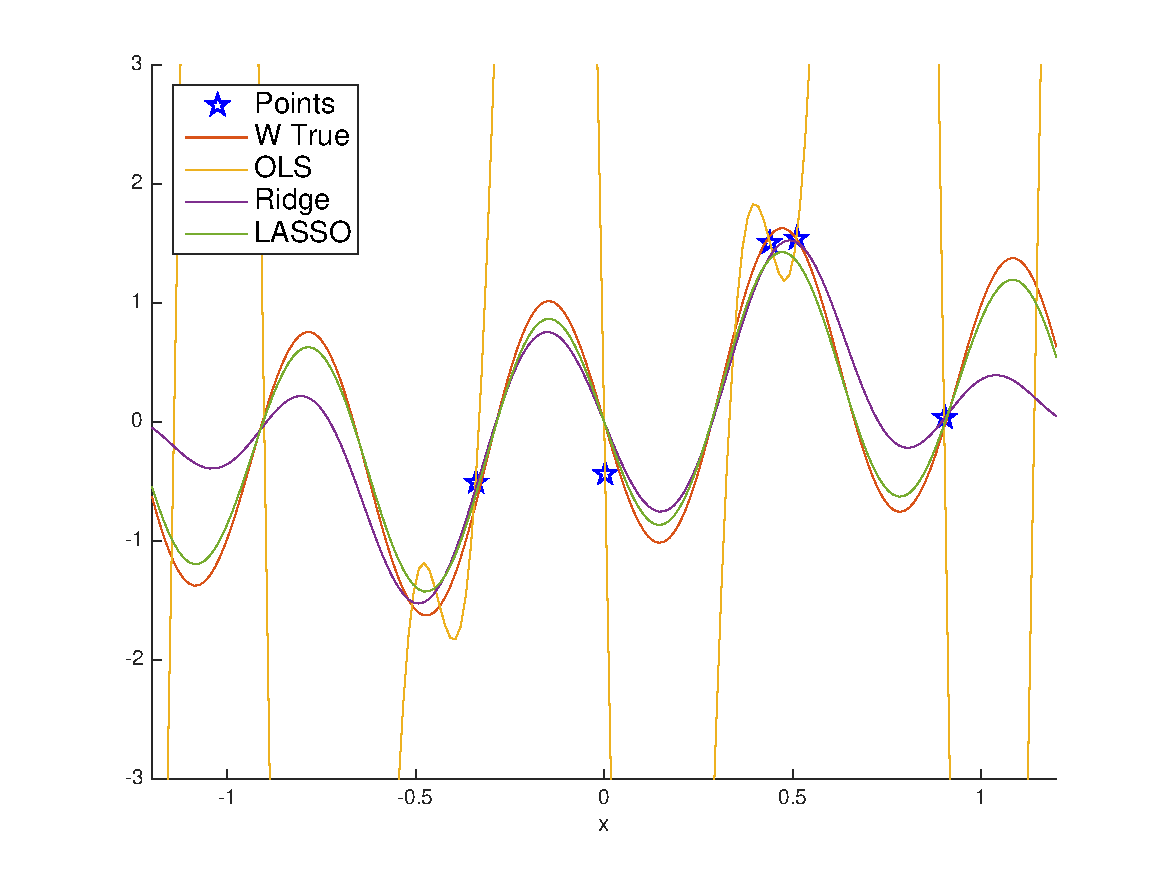
\includegraphics[scale=0.8]{hw1_4_1.pdf}
\caption{Plots of estimated function with different regularizers. \\
OLS: $\lambda_1 = \lambda_2 = 0$, Ridge: $\lambda_2 = 0.1$, LASSO: $\lambda_1 = 0.1$.} \label{fig:lasso_sparsity}
\end{figure}

\end{document}